\documentclass{article} % For LaTeX2e
\usepackage{iclr2021_conference,times}

% Optional math commands from https://github.com/goodfeli/dlbook_notation.
%%%%% NEW MATH DEFINITIONS %%%%%

\usepackage{amsmath,amsfonts,bm}

% Mark sections of captions for referring to divisions of figures
\newcommand{\figleft}{{\em (Left)}}
\newcommand{\figcenter}{{\em (Center)}}
\newcommand{\figright}{{\em (Right)}}
\newcommand{\figtop}{{\em (Top)}}
\newcommand{\figbottom}{{\em (Bottom)}}
\newcommand{\captiona}{{\em (a)}}
\newcommand{\captionb}{{\em (b)}}
\newcommand{\captionc}{{\em (c)}}
\newcommand{\captiond}{{\em (d)}}

% Highlight a newly defined term
\newcommand{\newterm}[1]{{\bf #1}}


% Figure reference, lower-case.
\def\figref#1{figure~\ref{#1}}
% Figure reference, capital. For start of sentence
\def\Figref#1{Figure~\ref{#1}}
\def\twofigref#1#2{figures \ref{#1} and \ref{#2}}
\def\quadfigref#1#2#3#4{figures \ref{#1}, \ref{#2}, \ref{#3} and \ref{#4}}
% Section reference, lower-case.
\def\secref#1{section~\ref{#1}}
% Section reference, capital.
\def\Secref#1{Section~\ref{#1}}
% Reference to two sections.
\def\twosecrefs#1#2{sections \ref{#1} and \ref{#2}}
% Reference to three sections.
\def\secrefs#1#2#3{sections \ref{#1}, \ref{#2} and \ref{#3}}
% Reference to an equation, lower-case.
\def\eqref#1{equation~\ref{#1}}
% Reference to an equation, upper case
\def\Eqref#1{Equation~\ref{#1}}
% A raw reference to an equation---avoid using if possible
\def\plaineqref#1{\ref{#1}}
% Reference to a chapter, lower-case.
\def\chapref#1{chapter~\ref{#1}}
% Reference to an equation, upper case.
\def\Chapref#1{Chapter~\ref{#1}}
% Reference to a range of chapters
\def\rangechapref#1#2{chapters\ref{#1}--\ref{#2}}
% Reference to an algorithm, lower-case.
\def\algref#1{algorithm~\ref{#1}}
% Reference to an algorithm, upper case.
\def\Algref#1{Algorithm~\ref{#1}}
\def\twoalgref#1#2{algorithms \ref{#1} and \ref{#2}}
\def\Twoalgref#1#2{Algorithms \ref{#1} and \ref{#2}}
% Reference to a part, lower case
\def\partref#1{part~\ref{#1}}
% Reference to a part, upper case
\def\Partref#1{Part~\ref{#1}}
\def\twopartref#1#2{parts \ref{#1} and \ref{#2}}

\def\ceil#1{\lceil #1 \rceil}
\def\floor#1{\lfloor #1 \rfloor}
\def\1{\bm{1}}
\newcommand{\train}{\mathcal{D}}
\newcommand{\valid}{\mathcal{D_{\mathrm{valid}}}}
\newcommand{\test}{\mathcal{D_{\mathrm{test}}}}

\def\eps{{\epsilon}}


% Random variables
\def\reta{{\textnormal{$\eta$}}}
\def\ra{{\textnormal{a}}}
\def\rb{{\textnormal{b}}}
\def\rc{{\textnormal{c}}}
\def\rd{{\textnormal{d}}}
\def\re{{\textnormal{e}}}
\def\rf{{\textnormal{f}}}
\def\rg{{\textnormal{g}}}
\def\rh{{\textnormal{h}}}
\def\ri{{\textnormal{i}}}
\def\rj{{\textnormal{j}}}
\def\rk{{\textnormal{k}}}
\def\rl{{\textnormal{l}}}
% rm is already a command, just don't name any random variables m
\def\rn{{\textnormal{n}}}
\def\ro{{\textnormal{o}}}
\def\rp{{\textnormal{p}}}
\def\rq{{\textnormal{q}}}
\def\rr{{\textnormal{r}}}
\def\rs{{\textnormal{s}}}
\def\rt{{\textnormal{t}}}
\def\ru{{\textnormal{u}}}
\def\rv{{\textnormal{v}}}
\def\rw{{\textnormal{w}}}
\def\rx{{\textnormal{x}}}
\def\ry{{\textnormal{y}}}
\def\rz{{\textnormal{z}}}

% Random vectors
\def\rvepsilon{{\mathbf{\epsilon}}}
\def\rvtheta{{\mathbf{\theta}}}
\def\rva{{\mathbf{a}}}
\def\rvb{{\mathbf{b}}}
\def\rvc{{\mathbf{c}}}
\def\rvd{{\mathbf{d}}}
\def\rve{{\mathbf{e}}}
\def\rvf{{\mathbf{f}}}
\def\rvg{{\mathbf{g}}}
\def\rvh{{\mathbf{h}}}
\def\rvu{{\mathbf{i}}}
\def\rvj{{\mathbf{j}}}
\def\rvk{{\mathbf{k}}}
\def\rvl{{\mathbf{l}}}
\def\rvm{{\mathbf{m}}}
\def\rvn{{\mathbf{n}}}
\def\rvo{{\mathbf{o}}}
\def\rvp{{\mathbf{p}}}
\def\rvq{{\mathbf{q}}}
\def\rvr{{\mathbf{r}}}
\def\rvs{{\mathbf{s}}}
\def\rvt{{\mathbf{t}}}
\def\rvu{{\mathbf{u}}}
\def\rvv{{\mathbf{v}}}
\def\rvw{{\mathbf{w}}}
\def\rvx{{\mathbf{x}}}
\def\rvy{{\mathbf{y}}}
\def\rvz{{\mathbf{z}}}

% Elements of random vectors
\def\erva{{\textnormal{a}}}
\def\ervb{{\textnormal{b}}}
\def\ervc{{\textnormal{c}}}
\def\ervd{{\textnormal{d}}}
\def\erve{{\textnormal{e}}}
\def\ervf{{\textnormal{f}}}
\def\ervg{{\textnormal{g}}}
\def\ervh{{\textnormal{h}}}
\def\ervi{{\textnormal{i}}}
\def\ervj{{\textnormal{j}}}
\def\ervk{{\textnormal{k}}}
\def\ervl{{\textnormal{l}}}
\def\ervm{{\textnormal{m}}}
\def\ervn{{\textnormal{n}}}
\def\ervo{{\textnormal{o}}}
\def\ervp{{\textnormal{p}}}
\def\ervq{{\textnormal{q}}}
\def\ervr{{\textnormal{r}}}
\def\ervs{{\textnormal{s}}}
\def\ervt{{\textnormal{t}}}
\def\ervu{{\textnormal{u}}}
\def\ervv{{\textnormal{v}}}
\def\ervw{{\textnormal{w}}}
\def\ervx{{\textnormal{x}}}
\def\ervy{{\textnormal{y}}}
\def\ervz{{\textnormal{z}}}

% Random matrices
\def\rmA{{\mathbf{A}}}
\def\rmB{{\mathbf{B}}}
\def\rmC{{\mathbf{C}}}
\def\rmD{{\mathbf{D}}}
\def\rmE{{\mathbf{E}}}
\def\rmF{{\mathbf{F}}}
\def\rmG{{\mathbf{G}}}
\def\rmH{{\mathbf{H}}}
\def\rmI{{\mathbf{I}}}
\def\rmJ{{\mathbf{J}}}
\def\rmK{{\mathbf{K}}}
\def\rmL{{\mathbf{L}}}
\def\rmM{{\mathbf{M}}}
\def\rmN{{\mathbf{N}}}
\def\rmO{{\mathbf{O}}}
\def\rmP{{\mathbf{P}}}
\def\rmQ{{\mathbf{Q}}}
\def\rmR{{\mathbf{R}}}
\def\rmS{{\mathbf{S}}}
\def\rmT{{\mathbf{T}}}
\def\rmU{{\mathbf{U}}}
\def\rmV{{\mathbf{V}}}
\def\rmW{{\mathbf{W}}}
\def\rmX{{\mathbf{X}}}
\def\rmY{{\mathbf{Y}}}
\def\rmZ{{\mathbf{Z}}}

% Elements of random matrices
\def\ermA{{\textnormal{A}}}
\def\ermB{{\textnormal{B}}}
\def\ermC{{\textnormal{C}}}
\def\ermD{{\textnormal{D}}}
\def\ermE{{\textnormal{E}}}
\def\ermF{{\textnormal{F}}}
\def\ermG{{\textnormal{G}}}
\def\ermH{{\textnormal{H}}}
\def\ermI{{\textnormal{I}}}
\def\ermJ{{\textnormal{J}}}
\def\ermK{{\textnormal{K}}}
\def\ermL{{\textnormal{L}}}
\def\ermM{{\textnormal{M}}}
\def\ermN{{\textnormal{N}}}
\def\ermO{{\textnormal{O}}}
\def\ermP{{\textnormal{P}}}
\def\ermQ{{\textnormal{Q}}}
\def\ermR{{\textnormal{R}}}
\def\ermS{{\textnormal{S}}}
\def\ermT{{\textnormal{T}}}
\def\ermU{{\textnormal{U}}}
\def\ermV{{\textnormal{V}}}
\def\ermW{{\textnormal{W}}}
\def\ermX{{\textnormal{X}}}
\def\ermY{{\textnormal{Y}}}
\def\ermZ{{\textnormal{Z}}}

% Vectors
\def\vzero{{\bm{0}}}
\def\vone{{\bm{1}}}
\def\vmu{{\bm{\mu}}}
\def\vtheta{{\bm{\theta}}}
\def\va{{\bm{a}}}
\def\vb{{\bm{b}}}
\def\vc{{\bm{c}}}
\def\vd{{\bm{d}}}
\def\ve{{\bm{e}}}
\def\vf{{\bm{f}}}
\def\vg{{\bm{g}}}
\def\vh{{\bm{h}}}
\def\vi{{\bm{i}}}
\def\vj{{\bm{j}}}
\def\vk{{\bm{k}}}
\def\vl{{\bm{l}}}
\def\vm{{\bm{m}}}
\def\vn{{\bm{n}}}
\def\vo{{\bm{o}}}
\def\vp{{\bm{p}}}
\def\vq{{\bm{q}}}
\def\vr{{\bm{r}}}
\def\vs{{\bm{s}}}
\def\vt{{\bm{t}}}
\def\vu{{\bm{u}}}
\def\vv{{\bm{v}}}
\def\vw{{\bm{w}}}
\def\vx{{\bm{x}}}
\def\vy{{\bm{y}}}
\def\vz{{\bm{z}}}

% Elements of vectors
\def\evalpha{{\alpha}}
\def\evbeta{{\beta}}
\def\evepsilon{{\epsilon}}
\def\evlambda{{\lambda}}
\def\evomega{{\omega}}
\def\evmu{{\mu}}
\def\evpsi{{\psi}}
\def\evsigma{{\sigma}}
\def\evtheta{{\theta}}
\def\eva{{a}}
\def\evb{{b}}
\def\evc{{c}}
\def\evd{{d}}
\def\eve{{e}}
\def\evf{{f}}
\def\evg{{g}}
\def\evh{{h}}
\def\evi{{i}}
\def\evj{{j}}
\def\evk{{k}}
\def\evl{{l}}
\def\evm{{m}}
\def\evn{{n}}
\def\evo{{o}}
\def\evp{{p}}
\def\evq{{q}}
\def\evr{{r}}
\def\evs{{s}}
\def\evt{{t}}
\def\evu{{u}}
\def\evv{{v}}
\def\evw{{w}}
\def\evx{{x}}
\def\evy{{y}}
\def\evz{{z}}

% Matrix
\def\mA{{\bm{A}}}
\def\mB{{\bm{B}}}
\def\mC{{\bm{C}}}
\def\mD{{\bm{D}}}
\def\mE{{\bm{E}}}
\def\mF{{\bm{F}}}
\def\mG{{\bm{G}}}
\def\mH{{\bm{H}}}
\def\mI{{\bm{I}}}
\def\mJ{{\bm{J}}}
\def\mK{{\bm{K}}}
\def\mL{{\bm{L}}}
\def\mM{{\bm{M}}}
\def\mN{{\bm{N}}}
\def\mO{{\bm{O}}}
\def\mP{{\bm{P}}}
\def\mQ{{\bm{Q}}}
\def\mR{{\bm{R}}}
\def\mS{{\bm{S}}}
\def\mT{{\bm{T}}}
\def\mU{{\bm{U}}}
\def\mV{{\bm{V}}}
\def\mW{{\bm{W}}}
\def\mX{{\bm{X}}}
\def\mY{{\bm{Y}}}
\def\mZ{{\bm{Z}}}
\def\mBeta{{\bm{\beta}}}
\def\mPhi{{\bm{\Phi}}}
\def\mLambda{{\bm{\Lambda}}}
\def\mSigma{{\bm{\Sigma}}}

% Tensor
\DeclareMathAlphabet{\mathsfit}{\encodingdefault}{\sfdefault}{m}{sl}
\SetMathAlphabet{\mathsfit}{bold}{\encodingdefault}{\sfdefault}{bx}{n}
\newcommand{\tens}[1]{\bm{\mathsfit{#1}}}
\def\tA{{\tens{A}}}
\def\tB{{\tens{B}}}
\def\tC{{\tens{C}}}
\def\tD{{\tens{D}}}
\def\tE{{\tens{E}}}
\def\tF{{\tens{F}}}
\def\tG{{\tens{G}}}
\def\tH{{\tens{H}}}
\def\tI{{\tens{I}}}
\def\tJ{{\tens{J}}}
\def\tK{{\tens{K}}}
\def\tL{{\tens{L}}}
\def\tM{{\tens{M}}}
\def\tN{{\tens{N}}}
\def\tO{{\tens{O}}}
\def\tP{{\tens{P}}}
\def\tQ{{\tens{Q}}}
\def\tR{{\tens{R}}}
\def\tS{{\tens{S}}}
\def\tT{{\tens{T}}}
\def\tU{{\tens{U}}}
\def\tV{{\tens{V}}}
\def\tW{{\tens{W}}}
\def\tX{{\tens{X}}}
\def\tY{{\tens{Y}}}
\def\tZ{{\tens{Z}}}


% Graph
\def\gA{{\mathcal{A}}}
\def\gB{{\mathcal{B}}}
\def\gC{{\mathcal{C}}}
\def\gD{{\mathcal{D}}}
\def\gE{{\mathcal{E}}}
\def\gF{{\mathcal{F}}}
\def\gG{{\mathcal{G}}}
\def\gH{{\mathcal{H}}}
\def\gI{{\mathcal{I}}}
\def\gJ{{\mathcal{J}}}
\def\gK{{\mathcal{K}}}
\def\gL{{\mathcal{L}}}
\def\gM{{\mathcal{M}}}
\def\gN{{\mathcal{N}}}
\def\gO{{\mathcal{O}}}
\def\gP{{\mathcal{P}}}
\def\gQ{{\mathcal{Q}}}
\def\gR{{\mathcal{R}}}
\def\gS{{\mathcal{S}}}
\def\gT{{\mathcal{T}}}
\def\gU{{\mathcal{U}}}
\def\gV{{\mathcal{V}}}
\def\gW{{\mathcal{W}}}
\def\gX{{\mathcal{X}}}
\def\gY{{\mathcal{Y}}}
\def\gZ{{\mathcal{Z}}}

% Sets
\def\sA{{\mathbb{A}}}
\def\sB{{\mathbb{B}}}
\def\sC{{\mathbb{C}}}
\def\sD{{\mathbb{D}}}
% Don't use a set called E, because this would be the same as our symbol
% for expectation.
\def\sF{{\mathbb{F}}}
\def\sG{{\mathbb{G}}}
\def\sH{{\mathbb{H}}}
\def\sI{{\mathbb{I}}}
\def\sJ{{\mathbb{J}}}
\def\sK{{\mathbb{K}}}
\def\sL{{\mathbb{L}}}
\def\sM{{\mathbb{M}}}
\def\sN{{\mathbb{N}}}
\def\sO{{\mathbb{O}}}
\def\sP{{\mathbb{P}}}
\def\sQ{{\mathbb{Q}}}
\def\sR{{\mathbb{R}}}
\def\sS{{\mathbb{S}}}
\def\sT{{\mathbb{T}}}
\def\sU{{\mathbb{U}}}
\def\sV{{\mathbb{V}}}
\def\sW{{\mathbb{W}}}
\def\sX{{\mathbb{X}}}
\def\sY{{\mathbb{Y}}}
\def\sZ{{\mathbb{Z}}}

% Entries of a matrix
\def\emLambda{{\Lambda}}
\def\emA{{A}}
\def\emB{{B}}
\def\emC{{C}}
\def\emD{{D}}
\def\emE{{E}}
\def\emF{{F}}
\def\emG{{G}}
\def\emH{{H}}
\def\emI{{I}}
\def\emJ{{J}}
\def\emK{{K}}
\def\emL{{L}}
\def\emM{{M}}
\def\emN{{N}}
\def\emO{{O}}
\def\emP{{P}}
\def\emQ{{Q}}
\def\emR{{R}}
\def\emS{{S}}
\def\emT{{T}}
\def\emU{{U}}
\def\emV{{V}}
\def\emW{{W}}
\def\emX{{X}}
\def\emY{{Y}}
\def\emZ{{Z}}
\def\emSigma{{\Sigma}}

% entries of a tensor
% Same font as tensor, without \bm wrapper
\newcommand{\etens}[1]{\mathsfit{#1}}
\def\etLambda{{\etens{\Lambda}}}
\def\etA{{\etens{A}}}
\def\etB{{\etens{B}}}
\def\etC{{\etens{C}}}
\def\etD{{\etens{D}}}
\def\etE{{\etens{E}}}
\def\etF{{\etens{F}}}
\def\etG{{\etens{G}}}
\def\etH{{\etens{H}}}
\def\etI{{\etens{I}}}
\def\etJ{{\etens{J}}}
\def\etK{{\etens{K}}}
\def\etL{{\etens{L}}}
\def\etM{{\etens{M}}}
\def\etN{{\etens{N}}}
\def\etO{{\etens{O}}}
\def\etP{{\etens{P}}}
\def\etQ{{\etens{Q}}}
\def\etR{{\etens{R}}}
\def\etS{{\etens{S}}}
\def\etT{{\etens{T}}}
\def\etU{{\etens{U}}}
\def\etV{{\etens{V}}}
\def\etW{{\etens{W}}}
\def\etX{{\etens{X}}}
\def\etY{{\etens{Y}}}
\def\etZ{{\etens{Z}}}

% The true underlying data generating distribution
\newcommand{\pdata}{p_{\rm{data}}}
% The empirical distribution defined by the training set
\newcommand{\ptrain}{\hat{p}_{\rm{data}}}
\newcommand{\Ptrain}{\hat{P}_{\rm{data}}}
% The model distribution
\newcommand{\pmodel}{p_{\rm{model}}}
\newcommand{\Pmodel}{P_{\rm{model}}}
\newcommand{\ptildemodel}{\tilde{p}_{\rm{model}}}
% Stochastic autoencoder distributions
\newcommand{\pencode}{p_{\rm{encoder}}}
\newcommand{\pdecode}{p_{\rm{decoder}}}
\newcommand{\precons}{p_{\rm{reconstruct}}}

\newcommand{\laplace}{\mathrm{Laplace}} % Laplace distribution

\newcommand{\E}{\mathbb{E}}
\newcommand{\Ls}{\mathcal{L}}
\newcommand{\R}{\mathbb{R}}
\newcommand{\emp}{\tilde{p}}
\newcommand{\lr}{\alpha}
\newcommand{\reg}{\lambda}
\newcommand{\rect}{\mathrm{rectifier}}
\newcommand{\softmax}{\mathrm{softmax}}
\newcommand{\sigmoid}{\sigma}
\newcommand{\softplus}{\zeta}
\newcommand{\KL}{D_{\mathrm{KL}}}
\newcommand{\Var}{\mathrm{Var}}
\newcommand{\standarderror}{\mathrm{SE}}
\newcommand{\Cov}{\mathrm{Cov}}
% Wolfram Mathworld says $L^2$ is for function spaces and $\ell^2$ is for vectors
% But then they seem to use $L^2$ for vectors throughout the site, and so does
% wikipedia.
\newcommand{\normlzero}{L^0}
\newcommand{\normlone}{L^1}
\newcommand{\normltwo}{L^2}
\newcommand{\normlp}{L^p}
\newcommand{\normmax}{L^\infty}

\newcommand{\parents}{Pa} % See usage in notation.tex. Chosen to match Daphne's book.

\DeclareMathOperator*{\argmax}{arg\,max}
\DeclareMathOperator*{\argmin}{arg\,min}

\DeclareMathOperator{\sign}{sign}
\DeclareMathOperator{\Tr}{Tr}
\let\ab\allowbreak


\usepackage{amsmath}
\usepackage{amssymb}
\usepackage{amsthm}
\usepackage{thmtools}
\usepackage{mathtools}
\usepackage{graphicx}
%\usepackage{algpseudocode}
%\usepackage{algorithm}
\usepackage[ruled,vlined,linesnumbered,algosection]{algorithm2e}
\usepackage{blindtext}
\usepackage{setspace}
\usepackage[utf8]{inputenc}
\usepackage[utf8]{vietnam}
\usepackage[center]{caption}
\usepackage[shortlabels]{enumitem}
\usepackage{fancyhdr} % header, footer
\usepackage{hyperref} % loại bỏ border với mục lục và công thức
\usepackage{url}
\usepackage[nonumberlist, nopostdot, nogroupskip]{glossaries}
\usepackage{glossary-superragged}
\usepackage{tikz,tkz-tab}
%\usepackage[style=numeric,sortcites]{biblatex}
%\addbibresource{ref.bib}
%\usepackage[numbers]{natbib}
\usepackage{indentfirst}
\usepackage{multirow}
\usepackage{cancel}

\graphicspath{{./figures/}}

\title{Mô hình sinh dựa trên điểm số bằng \\ phương trình vi phân ngẫu nhiên}


\author{Nguyễn Chí Thanh \\
Khoa Toán - Cơ - Tin học\\
Trường Đại học Khoa học Tự nhiên\\
Đại học Quốc Gia Hà Nội \\
\texttt{nguyenchithanh\_sdh21@hus.edu.vn} \\
}

\newcommand{\fix}{\marginpar{FIX}}
\newcommand{\new}{\marginpar{NEW}}

\iclrfinalcopy % Uncomment for camera-ready version, but NOT for submission.

\begin{document}
\maketitle

\begin{abstract}
    Tạo nhiễu từ dữ liệu là một việc đơn giản, nhưng tạo dữ liệu từ nhiễu được gọi là mô hình sinh.
    Ở đề tài này, ta sẽ trình bày phương trình vi phân ngẫu nhiên (SDE) biến đổi một phân phối dữ liệu phức tạp thành một phân phối tiên nghiệm biết trước trơn và thông suốt bằng cách dần dần thêm nhiễu vào dữ liệu,
    và một phương trình vi phân ngẫu nhiên (SDE) ngược (theo thời gian) biến đổi từ phân phối tiên nghiệm trở lại phân phối dữ liệu một cách từ từ bằng việc loại bỏ dần nhiễu.
    Một điều quan trọng là phương trình vi phân ngược theo thời gian chỉ phụ thuộc vào trường gradient phụ thuộc vào thời gian (được gọi là điểm số) của phân phối dữ liệu bị xáo trộn bởi nhiễu.
    Bằng việc tận dụng những bước tiến trong mô hình sinh dựa trên điểm, ta có thể ước lượng chính xác điểm với mạng neuron, và sử dụng các bộ giải phương trình vi phân ngẫu nhiên (SDE) bằng phương pháp số để sinh ra các mẫu dữ liệu.
    Ta sẽ chỉ ra rằng khung làm việc này bao gồm các cách tiếp cận trước đây về mô hình sinh dựa trên điểm số và các mô hình khuếch tán xác suất, cho phép các thủ tục mới để sinh dữ liệu ra đời với những khả năng mạnh hơn.
    Đặc biệt, ta sẽ giới thiệu một bộ dự đoán - căn chỉnh để căn chỉnh sai lệch trong quá trình biến đổi của phương trình vi phân ngẫu nhiên ngược thời gian được rời rạc hóa.
    Ta cũng thu được một mạng neuron ODE tương đương được lấy mẫu từ cùng phân phối như SDE, nhưng ngoài ra cũng cho phép tính toán chính xác độ hợp lý, và cải thiện độ hiệu quả của quá trình lấy mẫu.
    Ngoài ra, ta cũng cung cấp một cách mới để giải các bài toán ngược với các mô hình dựa trên điểm số, được giải thích với các thí nghiệm trên sinh mẫu dựa trên điều kiện nhãn, vẽ ảnh và tô màu.
    Kết hợp với nhiều bước tiến về các kiến trúc mô hình, ta đã đạt kỷ lục với việc sinh ảnh trên tập CIFAR-10 với điểm Inception score là 9.89 và FID là 2.20 và độ hợp lý rất tốt 2.99 bits/dim, và thể hiện khả năng sinh ảnh chân thực với ảnh có độ phân giải 1024 $\times$ 1024 lần đầu tiên từ một mô hình sinh dựa trên điểm số.
\end{abstract}

\section{GIỚI THIỆU}

Hai lớp thành công của các mô hình sinh xác suất liên quan đến việc làm biến đổi dữ liệu một cách tuần tự với độ nhiễu tăng dần, sau đó học cách đảo ngược sự biến đổi để tạ thành một mô hình sinh của dữ liệu.
\textit{Score matching with Langevin dynamics} (SMLD) \citep{song2019generative} ước lượng điểm số (ví dụ gradient của log của hàm mật độ xác suất của dữ liệu) tại từng mức nhiễu, sau đó sử dụng động học Langevin để lấy mẫu từ mỗi dãy các mức nhiễu giảm dần trong suốt quá trình sinh dữ liệu.
\textit{Denoising diffusion probabilistic modeling} (DDPM) \citep{sohl2015deep,ho2020denoising} huấn luyện một dãy các mô hình xác suất để đảo ngược từng bước của quá trình bị xáo trộn bởi nhiễu,
sử dụng những kiến thức về dạng chức năng của các phân phối ngược làm cho quá trình huấn luyện dễ dàng hơn.
Trong không gian trạng thái liên tục, DDPM huấn luyện hàm mục tiêu ngầm tính điểm số tại từng mức nhiễu.
Vì vậy, ta gọi hai lớp mô hình này là các \textit{mô hình sinh dựa trên điểm số}.

Các mô hình sinh dựa trên điểm số và các kỹ thuật liên quan \citep{bordes2017learning, goyal2017variational,du2019implicit} đã được chứng minh là hiệu quả trong bài toán sinh ảnh \citep{song2019generative,song2020sliced,ho2020denoising}, âm thanh \citep{chen2020wavegrad,kong2020diffwave}, đồ thị \citep{niu2020permutation} và các khối hình \citep{cai2020learning}.
Để cho phép các phương pháp lấy mẫu mới mở rộng khả năng của các mô hình sinh dựa trên điểm số, ta đề xuất một khung làm việc thống nhất tổng quát hóa các cách tiếp cận trước đó thông qua góc nhìn của phương trình vi phân ngẫu nhiên.

\begin{figure}[h!]
    \centering
    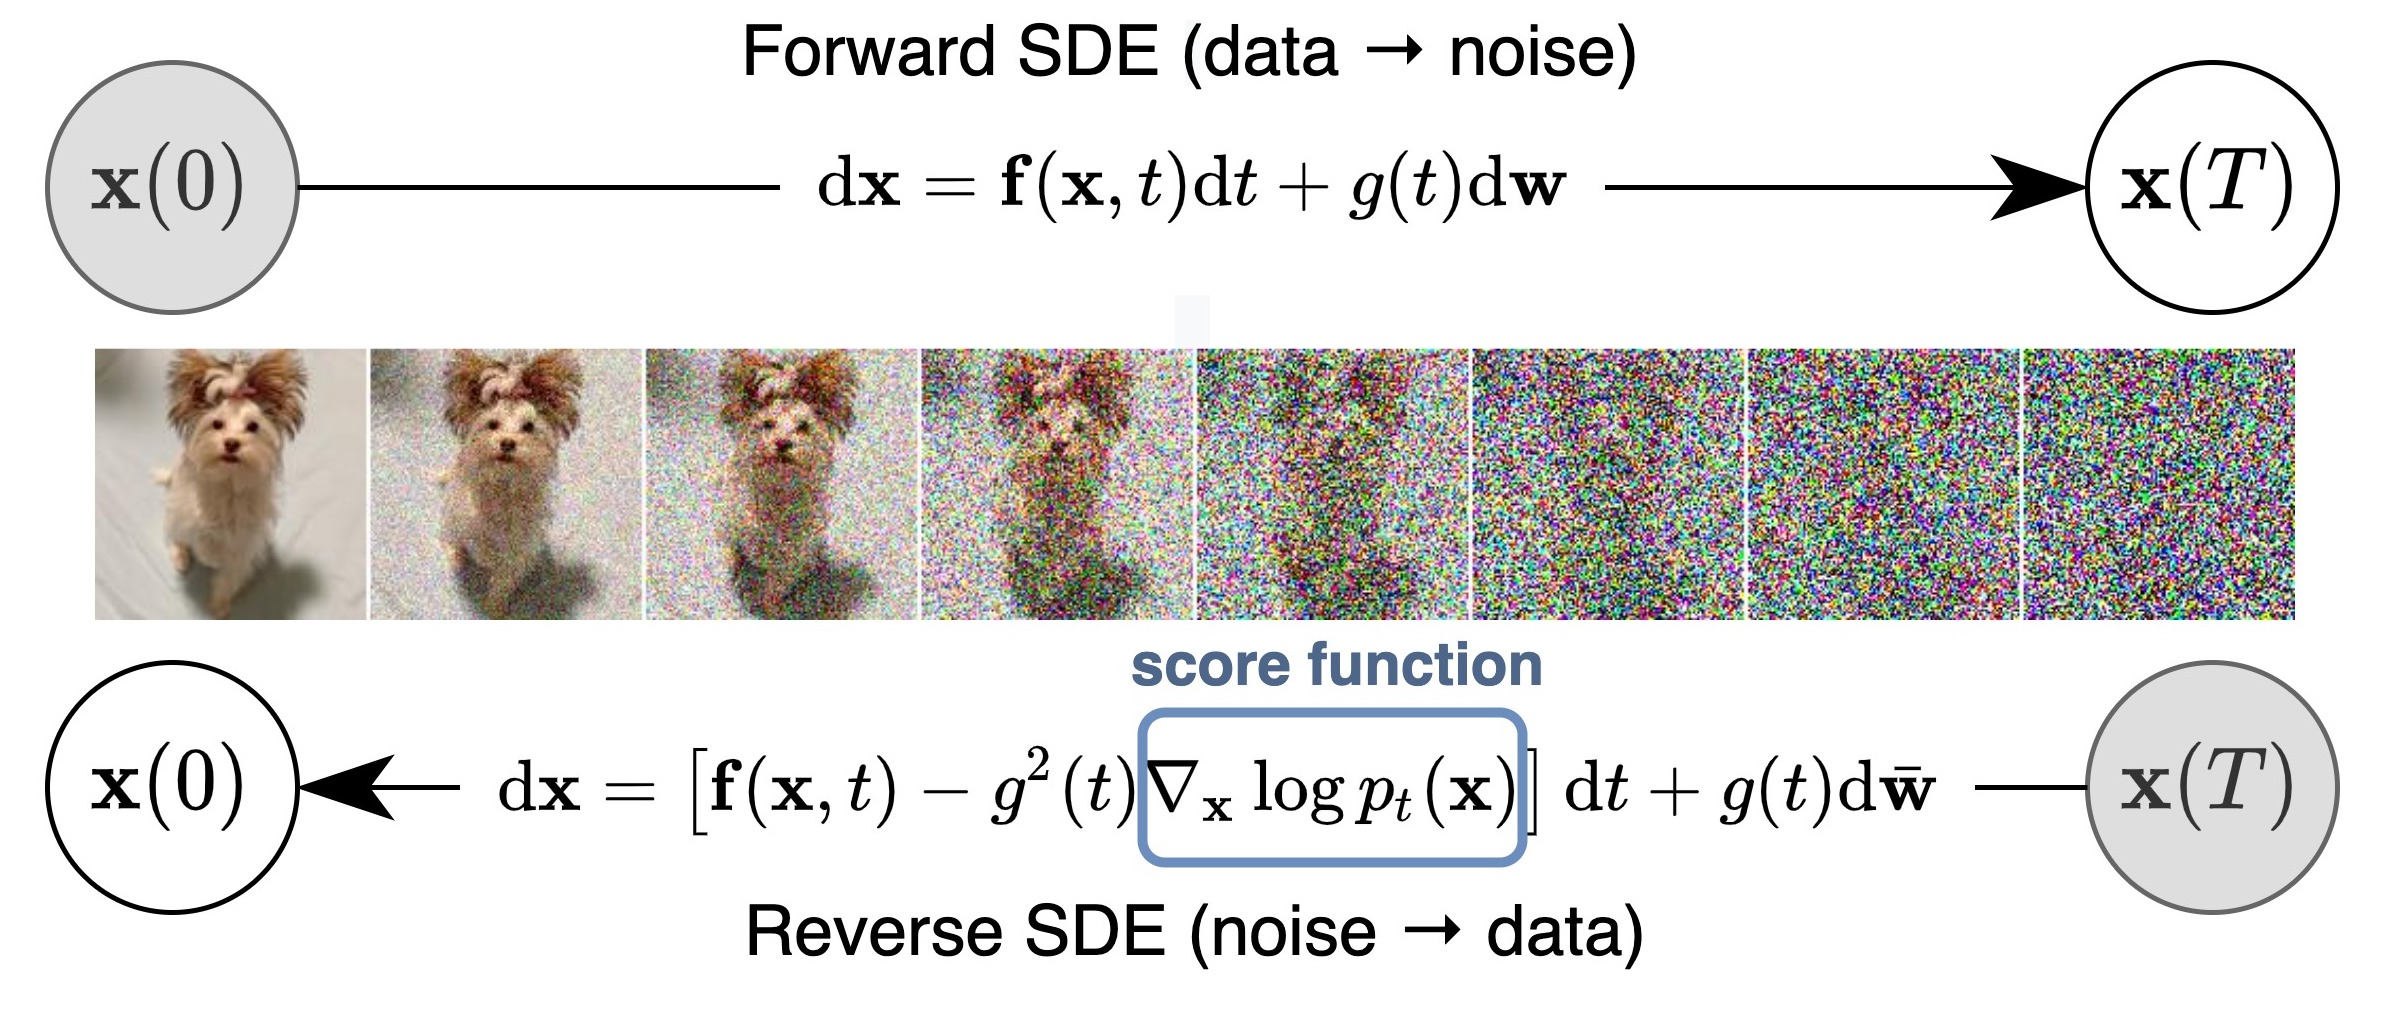
\includegraphics[width=0.8\textwidth]{1.jpg}
    \caption{\textbf{Giải một phương trình SDE đảo ngược thời gian thu được một mô hình sinh dựa trên điểm.}
    Biến đổi dữ liệu thành một phân phối nhiễu đơn giản có thể được thực hiện với một phương trình SDE liên tục theo thời gian.
    Phương trình SDE này có thể được đảo ngược nếu ta biết điểm của phân phối tại từng bước thời gian trung gian, $\nabla_{\bold{x}}\log p_t (\bold{x})$.}
    \label{fig:1}
\end{figure}

Cụ thể, thay vì làm nhiễu với một số hữu hạn của các phân phối nhiễu, ta xét một phân phối biến đổi một cách liên tục theo thời gian tương ứng với quá trình khuếch tán.
Quá trình này khuếch tán dần dần các điểm dữ liệu thành nhiễu ngẫu nhiên và được cho bởi một SDE cho trước không phụ thuộc vào dữ liệu và không có các tham số có thể huấn luyện.
Bằng cách đảo ngược quá trình này, ta có thể biến đổi nhiễu thành dữ liệu một cách trơn cho bài toán sinh mẫu dữ liệu.
Điều quan trọng là quá trình ngược này thỏa mãn SDE ngược theo thời gian \citep{anderson1982reverse}, có thể suy ra từ phương trình SDE thuận được cho bởi điểm số của hàm mật độ xác suất cận biên như là một hàm của thời gian.
Vì vậy ta có thể xấp xỉ SDE ngược thời gian bằng cách huấn luyện một mạng neuron phụ thuộc thời gian để ước lượng điểm số và sau đó tạo ra các mẫu dữ liệu sử dụng các bộ giải SDE bằng phương pháp số.
Ý tưởng chính được trình bày ở hình \ref{fig:1}.

Khung làm việc đề xuất có nhiều đóng góp về mặt lý thuyết và thực tiễn:

\textbf{Lấy mẫu linh hoạt và tính toán độ hợp lý:} Ta có thể sử dụng bất kỳ một bộ giải phương trình SDE đa chức năng nào để tích hợp phương trình SDE đảo ngược thời gian cho bài toán lấy mẫu.
Hơn nữa, ta đề xuất hai phương pháp đặc biệt mà không phù hợp với phương trình SDE nói chung: (i) Bộ lấy mẫu Dự đoán - Căn chỉnh (PC) kết hợp với bộ giải SDE bằng phương pháp số và cách tiếp cận MCMC (Markov Chain Monte Carlo) dựa trên điểm số, như Langevin MCMC \citep{parisi1981correlation} và HMC \citep{neal2011mcmc} và (ii) các bộ lấy mẫu tất định dựa trên dòng xác suất của các phương trình vi phân thường (ODE).
Phương pháp thứ nhất hợp nhất vả cải thiện các phương pháp lấy mẫu hiện có cho các mô hình dựa trên điểm số.
Phương pháp thứ hai cho phép lấy mẫu thích ứng nhanh thông qua một hộp đen là một bộ giải phương trình ODE, các thao tác trên dữ liệu linh hoạt thông qua mã ẩn, mỗi mã có tính duy nhất và điều đáng chú ý ta có thể tính chính xác độ hợp lý.

\textbf{Sinh dữ liệu có điều kiện:} Ta có thể điều chỉnh quá trình sinh dữ liệu bằng cách điều chỉnh các thông tin không có sẵn trong quá trình huấn luyện, bởi vì phương trình SDE đảo ngược thời gian có điều kiện có thể được ước lượng hiệu quả từ các điểm số \textit{không có điều kiện}.
Điều này cho phép các ứng dụng như sinh ảnh có điều kiện về lớp, vẽ ảnh, tô màu cũng như các bài toán ngược khác, tất cả các bài toán trên đều có thể được giải quyết bằng cách sử dụng một mô hình dựa trên điểm số không có điều kiện mà không cần phải huấn luyện lại mô hình.

\textbf{Khung làm việc thống nhất:} Khung làm việc của ta cung cấp một cách thống nhất để khai phá của chỉnh định nhiều phương trình SDE cho việc cải thiện các mô hình sinh dựa trên điểm số.
Các phương pháp của SMLD và DDPM có thể được đưa vào khung làm việc của ta bằng cách rời rạc hóa hai phương trình SDE riêng biệt.
Mặc dù DDPM \citep{ho2020denoising} gần đây đã được báo cáo là có thể đạt được mẫu có chất lượng cao hơn SMLD \citep{song2019generative,song2020improved}, ta chỉ ra điều đó với kiến trúc mạng tốt hơn và các thuật toán lấy mẫu mới cho phép bởi khung làm việc của ta, mô hình sau đó có thể bắt kịp và đạt được đến điểm Inception kỷ lục (9.89) và FID (2.20) trên tập CIFAR-10 cũng như độ chân thực của ảnh có độ phân giải 1024 $\times$ 1024 lần đầu tiên từ một mô hình sinh dựa trên điểm.
Ngoài ra, ta đề xuất một phương trình SDE mới trong khung làm việc của ta thu được độ hợp lý có giá trị 2.99 bits/dim trên tập CIFAR-10, tạo nên một kỷ lục mới cho bài toán này.

\section{Kiến thức nền tảng}

\subsection{Khử nhiều khớp điểm số với động học Langevin (SMLD)}

Đặt $p_{\sigma}(\tilde{\bold{x}} \vert \bold{x}) \vcentcolon = \mathcal{N}(\tilde{\bold{x}};\bold{x}, \sigma^2 \bold{I})$ là một nhân tạo ra nhiễu, và $p_{\sigma}(\tilde{\bold{x}})\vcentcolon = \int p_{\mathrm{data}}(\bold{x}) p_{\sigma}(\tilde{\bold{x}} \vert \bold{x}) d \bold{x}$, với $p_{\mathrm{data}}$ ký hiệu là phân phối dữ liệu.
Ta xét một dãy các mức nhiễu dương $\sigma_{\min} < \sigma_2 < \dots < \sigma_N = \sigma_{\max}$.
Thông thường, $\sigma_{\min}$ đủ nhỏ dể $p_{\sigma_{\min}} \approx p_{\mathrm{data}}(\bold{x})$, và $\sigma_{\max}$ đủ lớn để $p_{\sigma_{\max}}\approx \mathcal{N}(\bold{x}; \bold{0}, \sigma_{\max}^2 \bold{I})$.
\citep{song2019generative} đề xuất huấn luyện một mạng điểm số có điều kiện nhiễu (Noise Conditional Score Network - NCSN), ký hiệu $\bold{s}_{\boldsymbol{\theta}}(\bold{x}, \sigma)$ với một tổng có trọng số của các hàm khớp điểm số khử nhiễu \citep{vincent2011connection}:

\begin{equation} \label{eq:1}
    \boldsymbol{\theta}^{\ast} = \argmin_{\boldsymbol{\theta}} \sum_{i=1}^N \sigma_i^2 \mathbb{E}_{p_{\mathrm{data}}(\bold{x})} \mathbb{E}_{p_{\sigma_i}(\tilde{\bold{x}} \vert \bold{x})} \big\lbrack \lVert \bold{s}_{\boldsymbol{\theta} (\tilde{\bold{x}}, \sigma_i)} - \nabla_{\tilde{\bold{x}}} \log p_{\sigma_i} (\tilde{\bold{x}} \vert \bold{x})  \rVert_2^2 \big\rbrack
\end{equation}

Khi được cho một dữ liệu và một mô hình có kích thước phù hợp, mô hình dựa trên điểm số tối ưu $\bold{s}_{\boldsymbol{\theta}^{\ast}}(\bold{x}, \sigma)$ khớp với $\nabla_{\bold{x}} \log p_{\sigma}(\bold{x})$ tại hầu hết vị trí với $\sigma \in \lbrace \sigma_i \rbrace_{i=1}^N$.
Để lấy mẫu, \citep{song2019generative} chạy M bước của Langevin MCMC để thu được mẫu dữ liệu cho lần lượt từng $p_{\sigma_i}(\bold{x})$:

\begin{equation}
    \bold{x}_i^m = \bold{x}_i^{m-1} + \epsilon_i \bold{s}_{\boldsymbol{\theta}^{\ast}} (\bold{x}_i^{m-1}, \sigma_i) + \sqrt{2 \epsilon_i} \bold{z}_i^m, m = 1, 2, \dots, M
\end{equation}

với $\epsilon_i > 0$ là độ dài bước và $\bold{z}_i^m$ là một biến tuân theo phân phối chuẩn tắc.
Công thức trên được lặp lại cho $i=N, N-1, \dots, 1$ với $\bold{x}_N^0 \sim \mathcal{N}(\bold{x} \vert \bold{0}, \sigma_{\max}^2 \bold{I})$ và $\bold{x}_i^0 = \bold{x}_{i+1}^M$ khi $i < N$. Khi $M \rightarrow \infty$ và $\epsilon_i \rightarrow 0$ với mọi $i, \bold{x}_1^M$ trở thành một mẫu chính xác từ $p_{\sigma_{\min}}(\bold{x})\approx p_{\mathrm{data}}(\bold{x})$ trong một số điều kiện.


\subsection{Mô hình xác suất khuếch tán khử nhiễu (DDPM)}

\citep{sohl2015deep,ho2020denoising} xét một dãy các ngưỡng nhiễu dương $0 < \beta_1, \beta_2, \dots, \beta_N < 1$.
Với từng điểm dữ liệu huấn luyện $\bold{x}_0 \sim p_{\mathrm{data}}(\bold{x})$, một xích Markov rời rạc $\lbrace \bold{x}_1, \bold{x}_2, \dots, \bold{x}_N \rbrace$ được tạo ra sao cho $p(\bold{x}_i \vert \bold{x}_{i-1}) = \mathcal{N}(\bold{x}_i; \sqrt{1-\beta_i} \bold{x}_{i-1}, \beta_i \bold{I})$ và vì vậy $p_{\alpha_i}=\mathcal{N}(\bold{x}_i; \sqrt{\alpha_i}\bold{x}_0, (1-\alpha_i)\bold{I})$,
với $\alpha_i \vcentcolon = \prod_{j=1}^i (1 - \beta_j)$.
Tương tự với SMLD, ta có thể ký hiệu phân phối dữ liệu bị xáo trộn là $p_{\alpha_i}\vcentcolon =  \int p_{\mathrm{data}}(\bold{x}) p_{\alpha_i}(\tilde{\bold{x}} \vert \bold{x}) d \bold{x}$.
Các mức nhiễu được chọn sao cho $\bold{x}_N$ có phân phối xấp xỉ phân phối chuẩn tắc $\mathcal{N}(\bold{0}, \bold{I})$.
Một xích Markov biến phân theo chiều ngược được tham số hóa với $p_{\boldsymbol{\theta}} (\bold{x}_{i-1} \vert \bold{x}_i)=\mathcal{N}\Big(\bold{x}_{i-1}; \dfrac{1}{\sqrt{1-\beta_i}}(\bold{x}_i + \beta_i \bold{s}_{\boldsymbol{\theta}}(\bold{x}_i, i)), \beta_i \bold{I}\Big)$ và được huấn luyện với một biến thể được đánh lại trọng số của cận dưới của độ hợp lý (ELBO):

\begin{equation} \label{eq:3}
    \boldsymbol{\theta}^{\ast} = \argmin_{\boldsymbol{\theta}} \sum_{i=1}^N (1 - \alpha_i) \mathbb{E}_{p_{\mathrm{data}}(\bold{x})} \mathbb{E}_{p_{\alpha_i (\tilde{\bold{x}} vert \bold{x})}} \big \lbrack \lVert \bold{s}_{\boldsymbol{\theta}} (\tilde{\bold{x}}, i) - \nabla_{\tilde{\bold{x}}} \log p_{\alpha_i} (\tilde{\bold{x}} \vert \bold{x}) \rVert_2^2 \big \rbrack
\end{equation}

Sau khi giải phương trình \ref{eq:3} để thu được mô hình tối ưu $\bold{s}_{\boldsymbol{\theta}^{\ast}}(\bold{x}, i)$, các mẫu có thể được tạo ra bằng cách bắt đầu từ một nhiễu tuân theo phân phối chuẩn tắc $\bold{x}_N \sim \mathcal{N}(\bold{0}, \bold{I})$ và sử dụng công thức ước lượng xích Markov ngược sau đây:

\begin{equation}
    \bold{x}_{i-1} = \dfrac{1}{\sqrt{1-\beta_i}} \big( \bold{x}_i + \beta_i \bold{s}_{\boldsymbol{\theta}^{\ast}} (\bold{x}_i, i) \big) + \sqrt{\beta_i} \bold{z}_i, i = N, N-1, \dots, 1
\end{equation}

Ta gọi phương pháp này là \textit{ancestral sampling}, khi mà phương pháp này thực hiện lấy mẫu từ một mô hình đồ thị $\prod_{i=1}^N p_{\boldsymbol{\theta}} (\bold{x}_{i-1} \vert \bold{x}_i)$.
Hàm mục tiêu trong công thức \ref{eq:3} là $L_{\mathrm{simple}}$ trong \citep{ho2020denoising} được viết dưới dạng khá tương đồng với công thức \ref{eq:1}.
Cũng như công thức \ref{eq:1}, công thức \ref{eq:3} cũng là tổng có trọng số của các hàm mục tiêu khớp điểm số khử nhiễu, $\nabla_{\bold{x}}\log p_{\alpha_i}(\bold{x})$.
Đáng chú ý là trọng số thứ $i$ được đề cập trong công thức \ref{eq:1} và công thức \ref{eq:3} là $\sigma_i^2$ và $(1-\alpha_i)$ liên quan đến các nhân gây xáo trộn tương ứng trong cùng một dạng chức năng:
$\sigma_i^2 \propto 1/\mathbb{E} \big \lbrack \lVert \nabla_{\bold{x}} \log p_{\sigma_i} (\tilde{\bold{x}} \vert \bold{x}) \rVert_2^2 \big \rbrack$ và $(1-\alpha_i) \propto 1/\mathbb{E} \big \lbrack \lVert \nabla_\bold{x} \log p_{\alpha_i}  (\tilde{\bold{x}} \vert \bold{x})\rVert_2^2 \big \rbrack$

\section{Mô hình sinh dựa trên điểm số với SDE}

Để làm nhiễu hay làm xáo trộn dữ liệu với nhiều mức nhiễu là một chìa khóa dẫn đến thành công của các phương pháp trước đây.
Ta đề xuất tổng quát hóa ý tưởng này hơn nữa trở thành một số vô hạn các mức nhiễu, chẳng hạn phân phối của dữ liệu bị làm nhiễu biến đổi tuân theo một phương trình SDE khi nhiễu tăng dần lên.
Tổng quát của khung làm việc của ta được miêu tả trong hình \ref{fig:2}


\begin{figure}[h!]
    \centering
    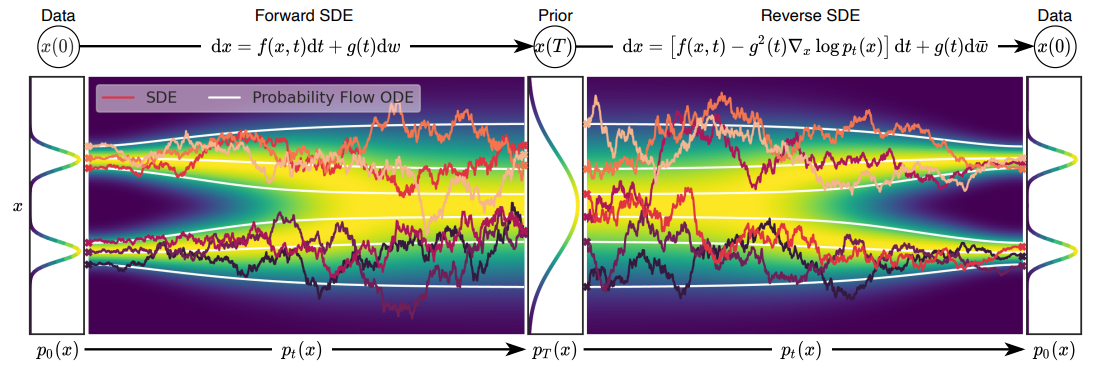
\includegraphics[width=\textwidth]{2.png}
    \caption{\textbf{Tổng quan của một mô hình sinh dựa trên điểm số với phương trình SDE}
    Ta có thể ánh xạ dữ liệu thành một phân phối nhiễu (phân phối tiên nghiệm) với một phương trình SDE (mục \ref{Pertubring-data-with-SDE}) và đảo ngược phương trình SDE này cho quá trình sinh dữ liệu (mục ).
    Ta cũng có thể đảo ngược dòng xác suất tương ứng phương trình ODE (mục ) thu được một quá trình tất định lấy mẫu từ cùng phân phối với SDE.
    Cả phương trình SDE đảo ngược thời gian và dòng xác suất phương trình ODE có thể đạt được bằng các ước lượng điểm số $\nabla_{\bold{x}} \log p_t (\bold{x})$ (mục \ref{Estimating-Scores-For-The-SDE}).}
    \label{fig:2}
\end{figure}

\subsection{Làm xáo trộn dữ liệu với phương trình SDE} \label{Pertubring-data-with-SDE}

Mục đích của ta là xây dựng một quá trình khuếch tán $\lbrace \bold{x}(t) \rbrace_{t=0}^T$ được đánh chỉ số bởi một biến thời gian liên tục $t \in \lbrack 0, T \rbrack$ ví dụ $\bold{x}(0) \sim p_0$, giả sử nếu ta có một bộ dữ liệu mà các điểm dữ liệu là độc lập và cùng phân phối, và $\bold{x}(T) \sim p_T$ là một dạng rất dễ xử lý để sinh các mẫu dữ liệu hiệu quả.
Hay nói cách khác, $p_0$ là phân phối dữ liệu và $p_T$ là phân phối tiên nghiệm.
Quá trình khuếch tán có thể được mô hình hóa là nghiệm của phương trình Ito SDE:

\begin{equation} \label{eq:5}
    d \bold{x} = \bold{f} (\bold{x}, t) dt + g(t) d \bold{w}
\end{equation}

với $\tilde{\bold{w}}$ là một quá trình Wiener chuẩn tắc (hay còn được gọi là chuyển Brown), $\bold{f}(.,t): \mathbb{R}^d \rightarrow \mathbb{R}^d$ là một hàm vector được gọi là hệ số độ trôi của $\bold{x}(t)$ và $g(.): \mathbb{R} \rightarrow \mathbb{R}$ là một hàm vô hướng được gọi là hệ số khuếch tán của $\bold{x}(t)$.
Để cho thuận tiện cho việc trình bày ta giả sử hệ số khuếch tán là một số vô hướng (thay vì là một ma trận $d \times d$) và không phụ thuộc vào $\bold{x}$, nhưng lý thuyết của ta có thể được tổng quát hóa và vẫn đúng trong trường hợp này (phụ lục ).
Phương trình SDE có một nghiệm riêng mạnh chừng nào các hệ số vẫn là Lipschitz toàn cục trong cả trạng thái và thời gian \citep{oksendal2003stochastic}.
Từ sau đây ta ký hiệu $p_t (\bold{x})$ là hàm mật độ xác suất của $\bold{x}(t)$ và sử dụng $p_{st}(\bold{x}(t) \vert \bold{x}(s))$ để ký hiệu nhân chuyển tiếp từ $\bold{x}(s)$ sang $\bold{x}(t)$, với $0 \leq s < s \leq T$.

Thông thường, $p_T$ là một phân phối phi cấu trúc không bao gồm thông tin nào của $p_0$, ví dụ như phân phối Gaussian với trung bình và phương sai cố định.
Có nhiều cách để thiết kế SDE trong phương trình \ref{eq:5} trong quá trình khuếch tán phân phối dữ liệu thành một phân phối tiên nghiệm cố định.
Ta cung cấp một số ví dụ trong mục  thu được quá trình tổng quát hóa liên tục của SMLD và DDPM.

\subsection{Sinh mẫu dữ liệu bằng cách đảo ngược phương trình SDE}

Ta bắt đầu từ các mẫu dữ liệu nhiễu $\bold{x}(T) \sim p_T$ và đảo ngược quá trình, ta có thể thu được các mẫu $\bold{x}(0) \sim p_0$.
Một kết quả đáng chú ý từ \citep{anderson1982reverse} chỉ ra rằng đảo ngược một quá trình khuếch tán cũng là một quá trình khuếch tán, đi ngược theo thời gian bởi một phương trình SDE đảo ngược thời gian:

\begin{equation} \label{eq:6}
    d \bold{x} = \big \lbrack \bold{f}(\bold{x}, t) - g(t)^2 \nabla_{\bold{x}} \log p_t (\bold{x}) \big \rbrack dt + g(t) d \hat{\bold{w}}
\end{equation}

với $\hat{\bold{w}}$ là một quá trình Wiener chuẩn tắc khi thời gian đi ngược từ $T$ về $0$, và $dt$ là một vi phân gia số thời gian âm.
Một khi điểm số của phân phối cận biên $\nabla_{\bold{x}} p_t(\bold{x})$ được biết với mọi $t$, ta có thể thu được quá trình khuếch tán ngược từ phương trình \ref{eq:6} và mô phỏng quá trình này để thu được mẫu dữ liệu từ phân phối $p_0$.

\subsection{Ước lượng điểm số cho phương trình SDE} \label{Estimating-Scores-For-The-SDE}

Điểm số của một phân phối có thể được ước lượng bằng cách huấn luyện một mô hình dựa trên điểm số trên các mẫu với khớp điểm số \citep{hyvarinen2005estimation,song2020sliced}. Để ước lượng $\nabla_{\bold{x}} \log p_t(\bold{x})$, ta có thể huấn luyện một mô hình dựa trên điểm số phụ thuộc vào thời gian $\bold{s}_{\boldsymbol{\theta}}(\bold{x}, t)$ thông qua một tổng quát hóa liên tục từ phương trình \ref{eq:1} và phương trình \ref{eq:3}:

\begin{equation} \label{eq:7}
    \boldsymbol{\theta}^{\ast} = \argmin_{\boldsymbol{\theta}} \mathbb{E}_t \Big \lbrace  \lambda(t) \mathbb{E}_{\bold{x}(0)} \mathbb{E}_{\bold{x}(t) \bold{x}(0)} \big \lbrack \lVert \bold{s}_{\boldsymbol{\theta}} (\bold{x}(t), t) - \nabla_{\bold{x}(t)} \log p_{0t} (\bold{x}(t) \vert \bold{x}(0)) \rVert_2^2 \big \lbrack \Big \rbrace
\end{equation}

với $\lambda: \lbrace 0, T \rbrace \rightarrow \mathbb{R}_{>0}$ là một hàm trọng số dương,
$t$ được lấy mẫu theo phân phối đều trên đoạn $\lbrace 0, T \rbrace$, $\bold{x}(0) \sim p_0 (\bold{x})$ và $\bold{x}(t) \sim p_{0t} (\bold{x}(t) \vert \bold{x}(0))$.
Với mô hình có kích thước và lượng dữ liệu phù hợp, khớp điểm số đảm bảo lời giải tối ưu của phương trình \ref{eq:7} được ký hiệu bởi $\bold{s}_{\boldsymbol{\theta}^{\ast}}(\bold{x}, t)$ bằng với $\nabla_{\bold{x}} \log p_t (\bold{x})$ với hầu hết $\bold{x}$ và $t$.
Trong SMLD và DDPM, ta thường chọn $\lambda \propto 1 / \mathbb{E} \big \lbrack \lVert \nabla_{\bold{x}(t)} \log p_{0t} (\bold{x}(t) \vert \bold{x}(0)) \rVert_2^2 \big \rbrack$.
Ta cần chú ý rằng công thức \ref{eq:7} sử dụng khớp điểm số khử nhiễu nhưng các hàm mục tiêu khớp điểm số khác ví dụ như khớp điểm số theo lát \citep{song2020sliced} và khớp điểm số sai phân hữu hạn \citep{pang2020efficient} cũng có thể được áp dụng ở đây.

Ta thường cũng cần phải biết nhân chuyển tiếp $p_{0t} (\bold{x}(t) \vert \bold{x}(0))$ để giải phương trình \ref{eq:7} một cách hiệu quả.
Nếu $\bold{f}(.,t)$ là hàm affine, nhân chuyển tiếp luôn luôn là phân phối Gaussian mà trung bình và phương sai thường được biết trong dạng đóng và có thể thu được bằng các kỹ thuật chuẩn tắc (xem mục 5.5  trong \cite{sarkka2019applied}).
Với phương trình SDE tổng quát hơn, ta có thể giải phương trình Kolmogorov thuận \citep{oksendal2003stochastic} để thu được $p_{0t} (\bold{x}(t) \vert \bold{x}(0))$.
Một cách khác, ta có thể mô phỏng phương trình SDE để lấy mẫu từ $p_{0t}(\bold{x}(t) \vert \bold{x}(0))$ và thay thế thành phần khớp điểm số khử nhiễu trong \ref{eq:7} với khớp điểm số theo lát để huấn luyện mô hình mà bỏ qua việc tính toán $\nabla_{\bold{x}(t)} \log p_{0t} (\bold{x}(t) \vert \bold{x}(0))$ (xem phụ lục ).

\subsection{Một số ví dụ: VE, VP SDE và các SDE khác}

Nhiễu được dùng để làm xáo trộn dữ liệu trong SMLD và DDPM có thể được xem là phiên bản rời rạc hóa của hai phương trình SDE khác nhau.
Ta sẽ nói ngắn gọn về phần này và chi tiết dudocj trình bày ở phụ lục .

Khi ta sử dụng $N$ mức nhiễu, từng nhân xáo trộn dữ liệu $p_{\sigma_i}(\bold{x} \vert \bold{x}_0)$ của SMLD tương ứng với phân phối của $\bold{x}_i$ theo xích Markov sau:

\begin{equation}
    \bold{x}_i = \bold{x}_{i-1} + \sqrt{\sigma_i^2 - \sigma_{i-1}^2} \bold{z}_{i-1}, i=1, \dots, N
\end{equation}

với $\bold{z}_{i-1} \sim \mathcal{N}(\bold{0}, \bold{I})$ và ta đã đặt $\sigma_0=0$ để làm đơn giản hóa ký hiệu.
Khi $N \rightarrow \infty$, $\lbrace \sigma_i \rbrace_{i=1}^N$ trở thành một hàm $\sigma(t)$, $\bold{z}_i$ trở thành $\bold{z}_t$, và xích Markov $\lbrace \bold{x}_i \rbrace_{i=1}^N$ trở thành một quá trình ngẫu nhiên liên tục $\lbrace \bold{x}(t) \rbrace_{t=0}^1$, ta sử dụng biến thời gian liên tục $t \in \lbrack 0, 1 \rbrack$ để đánh chỉ số thay vì số nguyên $i$.
Quá trình $\lbrace \bold{x}(t) \rbrace_{t=0}^1$ được cho bởi phương trình SDE sau:

\begin{equation} \label{eq:9}
    d \bold{x} = \sqrt{\dfrac{d \lbrack \sigma^2(t) \rbrack}{dt}} d \bold{w}
\end{equation}

Tương tự như với nhân gây xáo trộn $\lbrace p_{\alpha_i} (\bold{x} \vert \bold{x}_0) \rbrace_{i=1}^N$ của DDPM, xích Markov rời rạc là:

\begin{equation} \label{eq:10}
    \bold{x}_i = \sqrt{1 - \beta_i} \bold{x}_{i-1} + \sqrt{\beta_i} \bold{z}_{i-1}, i=1,\dots,N
\end{equation}

Khi $N \rightarrow \infty$, phương trình \ref{eq:10} hội tụ về phương trình SDE sau đây:

\begin{equation} \label{eq:11}
    d \bold{x} = \dfrac{1}{2} \beta(t) \bold{x} dt + \sqrt{\beta(t)} d\bold{w}
\end{equation}

\newpage
\bibliography{iclr2021_conference}
\bibliographystyle{iclr2021_conference}

\end{document}